\documentclass[xelatex,ja=standard,a4paper,14pt,everyparhook=compat]{bxjsarticle}
\usepackage{amsmath, amssymb, amsthm}
\usepackage{mathtools, bm}
\usepackage{enumitem}
\setenumerate{label=\alph*.}

% \usepackage{concmath}
% \usepackage[OT1]{fontenc}
\setsansfont{Segoe UI}
% \setmainfont{CMU Concrete}
% \usepackage{zxjatype}
\usepackage[noto-jp,oneweight]{zxjafont}
% \setCJKmainfont{Noto Serif JP}
% \setCJKsansfont{Noto Sans JP}

\usepackage{fancyhdr}
\pagestyle{fancy}
\lhead{\nouppercase{\leftmark}}
\rhead{\nouppercase{\rightmark}}
\renewcommand{\footrulewidth}{0.4pt}
\let\origtitle\title
\renewcommand{\title}[1]{\lfoot{#1}\origtitle{#1}}
\cfoot{}
\rfoot{\thepage}

\newcommand{\paren}[1]{\left(#1\right)}

\newcommand{\bbC}{\mathbb{C}}
\newcommand{\bbR}{\mathbb{R}}
\newcommand{\bbN}{\mathbb{N}}
\newcommand{\bbP}{\mathbb{P}}
\newcommand{\bbF}{\mathbb{F}}
\newcommand{\frakS}{\mathfrak{S}}
\newcommand{\mcA}{\mathcal{A}}
\DeclareMathOperator{\inv}{inv}
\DeclareMathOperator{\conv}{conv}
\DeclareMathOperator{\image}{Im}
\DeclareMathOperator{\rank}{rank}
\DeclareMathOperator{\ess}{ess}
\DeclareMathOperator{\codim}{codim}

\theoremstyle{definition}
\newtheorem{theorem}{定理}
\newtheorem*{theorem*}{定理}
\newtheorem{lemma}{補題}
\newtheorem*{lemma*}{補題}
\newtheorem{example}[theorem]{例}
\newtheorem*{example*}{例}
\newtheorem{definition}[theorem]{定義}
\newtheorem*{definition*}{定義}
\newtheorem{proposition}[theorem]{命題}
\newtheorem*{proposition*}{命題}
\newtheorem{corollary}[theorem]{系}
\newtheorem*{corollary*}{系}
\newtheorem{problem}{問題}
\newtheorem*{answer}{解答}
\renewcommand{\proofname}{\textup{証明}}

\usepackage{tcolorbox}
\tcbuselibrary{breakable,skins,theorems}

\tcolorboxenvironment{definition}{
    coltitle = black,
    % colback = white,
    colframe = green!35!black,
    fonttitle = \bfseries,
    breakable = true
}

\tcolorboxenvironment{definition*}{
    coltitle = black,
    % colback = white,
    colframe = green!35!black,
    fonttitle = \bfseries,
    breakable = true
}

\tcolorboxenvironment{theorem}{
    coltitle = black,
    % colback = black!10!white,
    colframe = blue!35!black,
    fonttitle = \bfseries,
    breakable = true
}

\tcolorboxenvironment{theorem*}{
    coltitle = black,
    % colback = black!10!white,
    colframe = blue!35!black,
    fonttitle = \bfseries,
    breakable = true
}

\tcolorboxenvironment{proposition}{
    coltitle = black,
    % colback = black!10!white,
    colframe = blue!35!black,
    fonttitle = \bfseries,
    breakable = true
}

\tcolorboxenvironment{proposition*}{
    coltitle = black,
    % colback = black!10!white,
    colframe = blue!35!black,
    fonttitle = \bfseries,
    breakable = true
}

\tcolorboxenvironment{corollary}{
    coltitle = black,
    % colback = black!10!white,
    colframe = blue!35!black,
    fonttitle = \bfseries,
    breakable = true
}

\tcolorboxenvironment{corollary*}{
    coltitle = black,
    % colback = black!10!white,
    colframe = blue!35!black,
    fonttitle = \bfseries,
    breakable = true
}

\tcolorboxenvironment{lemma}{
    coltitle = black,
    % colback = black!10!white,
    colframe = green!35!black,
    fonttitle = \bfseries,
    breakable = true
}

\tcolorboxenvironment{example}{
    coltitle = black,
    colback = white,
    colframe = purple!35!black,
    fonttitle = \bfseries,
    breakable = true
}

\tcolorboxenvironment{example*}{
    coltitle = black,
    colback = white,
    colframe = purple!35!black,
    fonttitle = \bfseries,
    breakable = true
}

\tcolorboxenvironment{lemma*}{
    coltitle = black,
    % colback = black!10!white,
    colframe = gray!35!black,
    fonttitle = \bfseries,
    breakable = true
}

\tcolorboxenvironment{proof}{
    blanker,
    breakable,
    left=5mm,
    before skip=10pt,
    after skip=10pt,
    borderline west={1mm}{0pt}{black}
}

\tcolorboxenvironment{proof*}{
    blanker,
    breakable,
    left=5mm,
    before skip=10pt,
    after skip=10pt,
    borderline west={1mm}{0pt}{black}
}

\tcolorboxenvironment{problem}{
    coltitle = black,
    % colback = black!10!white,
    colframe = black!35!black,
    fonttitle = \bfseries,
    breakable = true
}

\tcolorboxenvironment{answer}{
    blanker,
    breakable,
    left=5mm,
    before skip=10pt,
    after skip=10pt,
    borderline west={1mm}{0pt}{black}
}

\title{3.10節,3.11節}
\author{shino16}
\date{\today}

\begin{document}

\maketitle

\tableofcontents

\newpage

\setcounter{section}{-1}
\section{復習}

\begin{corollary*}[3.9.3,Weisnerの定理]
    $\#L \geq 2$の有限束$L$から$a \in L \setminus \{\hat1\}$をとると, \begin{equation*}
        \sum_{t : t \land a = \hat0} \mu(t, \hat1) = 0.
    \end{equation*}
\end{corollary*}
\begin{proof}
    (概略) $s \cdot t = s \land t$のもと$L$が成す$K$上の半群代数$A(L,K)$にて,
    \begin{equation*}
        \delta_t \coloneqq \sum_{s \leq t} \mu(s,t) s.
    \end{equation*}
    M\"obius反転より$a = \sum_{b \leq a} \delta_b$.また$\{\delta_t : t \in L\}$は$A(L,K)$の直交基底.

    \begin{equation*}
        a \delta_{\hat1} = \paren{\sum_{b \leq a} \delta_b} \delta_{\hat1} = 0,
    \end{equation*}
    \begin{equation*}
        a \delta_{\hat1} = a \sum_t \mu(t,\hat1) t = \sum_t \mu(t,\hat1) (a \land t),
    \end{equation*}
    にて$\hat0$の係数を比較して結果を得る.
\end{proof}

\begin{proposition*}[3.10.1]
    有限半モジュラ束$L$について,$(-1)^{\ell(s,t)}\mu(s,t) \geq 0$.
\end{proposition*}
\begin{proof}
    (概略) $L=[s,t]$とおき直し,原子$a$をとる.$t \land a = \hat0$ $\Leftrightarrow$ $t = \hat1$ or $t:\text{補原子}$より \begin{equation}
        \mu(\hat0,\hat1) = -\sum_{\text{補原子$t \not\geq a$}} \mu(\hat0, t).
    \end{equation}
    各$[\hat0,t]$はランクが$1$減った有限半モジュラ束なので,帰納法.
\end{proof}

\section{半モジュラ束$\Pi_n$とM\"obius関数}

有限集合$S$について,$\Pi_S \coloneqq \{\pi : \text{$S$の分割}\}$は \begin{equation*}
    \pi \leq \sigma \overset{\mathrm{def}}{\Longleftrightarrow} \text{$\pi$は$\sigma$の細分}
\end{equation*}
のもと半順序集合を成す.$\Pi_n \coloneqq \Pi_{[n]}$ ($[n] = \{1,\ldots,n\}$).
\begin{figure}[h]
    \centering
    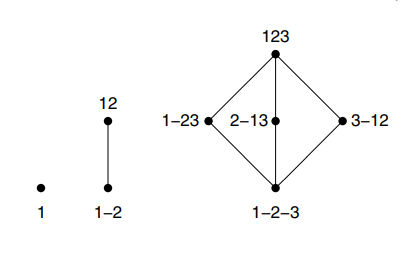
\includegraphics[width=.5\textwidth]{Fig3.20.png}
    \caption{Fig 3.20,左から$\Pi_1,\Pi_2,\Pi_3$}
\end{figure}

$\Pi_n$のランク関数は \begin{equation*}
    \rho(\pi) = n - \#\pi = n - (\text{$\pi$のブロック数}),
\end{equation*}
ランク母関数は \begin{equation*}
    F(\Pi_n, x) = \sum_{\pi \in \Pi_n} x^{\rho(\pi)} = \sum_{k=0}^{n-1} S(n,n-k) x^k.
\end{equation*}
(第二種Stirling数 $S(n,k) \coloneqq (\text{$[n]$の$k$ブロックへの分割の個数})$)

\newpage

\subsection{$\Pi_n$の特徴}

\begin{lemma*}
    $\Pi_n$は束(i.e.任意の$\pi,\sigma \in \Pi_n$について$\pi \land \sigma, \pi \lor \sigma$が存在).
\end{lemma*}
\begin{proof}
    $\pi \land \sigma$は簡単.$\pi, \sigma \leq [n]$なので,$\pi, \sigma$の上界全体の交わりをとって$\pi \lor \sigma$とできる.\footnote{命題3.3.1:有限交わり半束が$\hat1$を持つなら束,の証明と同じ議論.}
\end{proof}

\begin{lemma*}
    $L$は幾何束.すなわち, \begin{enumerate}
        \item $L$は有限半モジュラ束($\pi,\sigma \gtrdot \pi \land \sigma$ $\Longrightarrow$ $\pi \lor \sigma \gtrdot \pi,\sigma$)\footnote{$\rho(\pi) + \rho(\sigma) \geq \rho(\pi \land \sigma) + \rho(\pi \lor \sigma)$と同値.},かつ
        \item $L$は原子的(任意の元が原子の結びで表せる).\footnote{a.のもとこれは$L$がrelatively complementedであることと同値.}
    \end{enumerate}
\end{lemma*}
\begin{proof}
    \begin{enumerate}
        \item $\pi,\sigma \gtrdot \pi \land \sigma$と仮定.

              $\tau = \{B_1,\ldots,B_k\} \coloneqq \pi \land \sigma$とすると,$[\tau,\hat1] \cong \Pi_k$.あとはよい.

        \item $\hat0 = 1|2|\cdots|n \in\Pi_n$から$i,j$ ($i \neq j$)のみをマージした原子$\tau_{ij}$を考える.

              $\pi$は$\tau_{ij}$ ($i,j$は$\pi$上で同じブロック)全体の結び.
    \end{enumerate}
\end{proof}

\subsection{$\mu(\sigma,\pi)$の観察}

$[\sigma,\pi]$を調べる.

\begin{lemma*}
    $\pi = \{B_1,\ldots,B_k\}$とし,$B_i$が$\sigma$で$\lambda_i$個のブロックに分割されるとき, \begin{equation*}
        [\sigma,\pi] \cong \Pi_{\lambda_1} \times \Pi_{\lambda_2} \times \cdots \times \Pi_{\lambda_k}.
    \end{equation*}
\end{lemma*}
\begin{proof}
    略.
\end{proof}

補題の条件が成り立つとき,
\begin{equation*}
    \mu_n \coloneqq \mu_{\Pi_n}(\hat0, \hat1)
\end{equation*}
とすると \begin{equation*}
    \mu(\sigma, \pi) = \mu_{\lambda_1} \mu_{\lambda_2} \cdots \mu_{\lambda_k}.
\end{equation*}
$\mu_n$だけでも求まればOK.

補原子$a \coloneqq 12\cdots(n-1) | n \in \Pi_n$に系3.9.3を適用しよう.

\begin{lemma*}
    $t \in \Pi_n$について,次は同値. \begin{enumerate}
        \item $t \land a = \hat0$,
        \item $t = \hat0$,またはブロック$\{i,n\}$ ($i \in [n-1]$)を含む原子.
    \end{enumerate}
\end{lemma*}
\begin{proof}
    $\Pi_n$における$\land$の性質よりよい.
\end{proof}

\begin{proposition*}
    \begin{equation*}
        \mu_n = (-1)^{n-1}(n-1)!.
    \end{equation*}
\end{proposition*}
\begin{proof}
    系3.9.3を適用する.$t \in \Pi_n$について,$t = \hat0$のとき$\mu(t,\hat1) = \mu_n$,$t$が原子のとき$\mu(t,\hat1) = \mu_{n-1}$.したがって \begin{equation*}
        \mu_n = -(n-1)\mu_{n-1}.
    \end{equation*}

    $\mu_1 = 1$ ($\mu_2 = -1$)から帰納法.
\end{proof}

なお,より一般的な結果として \begin{equation*}
    \sum_{\pi \in \Pi_n} \mu(\hat0,\pi) x^{\#\pi} = (x)_n = x(x-1)\cdots(x-n+1).
\end{equation*}
これは後の章で証明される.

\subsection{特性方程式とWhitney数}

$P$:有限半順序集合,$\hat0$を持つ,階層的,ランク$n$

について\textbf{特性多項式}$\chi_P(x)$を次で定める: \begin{equation*}
    \chi_P(x) \coloneqq \sum_{t \in P} \mu(\hat0, t) x^{n-\rho(t)}.
\end{equation*}
ここで \begin{equation*}
    w_k \coloneqq [x^{n-k}]\chi_P(x) = \sum_{\substack{t \in P \\ \rho(t) = k}} \mu(\hat0,t)
\end{equation*}
は$k$番目の\textbf{第一種Whitney数}.$P=\Pi_n$のとき \begin{align*}
    \chi_{\Pi_n}(x) & = \sum_{\pi \in \Pi_n} \mu(\hat0,\pi)x^{(n-1)-\rho(\pi)} \\
                    & = (x-1)(x-2)\cdots(x-n+1).
\end{align*}
$\Pi_n$のランク$\ell(\Pi_n) = n-1$,$\rho(\pi) = n - \#\pi$に注意.このとき \begin{equation*}
    w_k = [x^{(n-1)-k}]\chi_{\Pi_n}(x) = s(n,n-k),
\end{equation*}
ただし$s$は第一種Stirling数.(組合せ的解釈ある?)

なお,ランク$k$の元$t \in P$の個数 \begin{equation*}
    W_k \coloneqq [x^k] F(P,x) = [x^k] \sum_{t \in P} x^{\rho(t)}
\end{equation*}
は$k$番目の\textbf{第二種Whitney数}.$P=\Pi_n$のとき$W_k = S(n,n-k)$.

% \subsection{余談:$s(n,k)$と$S(n,k)$の関係}

% \setcounter{problem}{129}
% \begin{problem}
%     有限半順序集合$P$が \begin{enumerate}[label=(\roman*)]
%         \item $P$は階層的でランク$n$,また$\hat0,\hat1$を持ち,かつ
%         \item 各$i = 0,\ldots,n$について, \begin{equation*}
%             \text{($\forall t \in P$) $\rho(t) = n-i$ $\Rightarrow$ $[t,\hat1] \cong Q_i$}
%         \end{equation*}
%         を満たす半順序集合$Q_i$が存在する,
%     \end{enumerate}
%     とする.このような$P$は\textbf{一様}であるという.

%     \begin{enumerate}
%         \item \begin{align*}
%             V(i,j) &\coloneqq \#\{t \in Q_i : \rho(t) = i-j\}, \\
%             v(i,j) &\coloneqq \sum_{\substack{t \in Q_i \\ \rho(t) = i-j}} \mu(\hat0,t),
%         \end{align*}
%         について,下三角行列$(V(i,j))_{0 \leq i,j \leq n},(v(i,j))_{0 \leq i,j \leq n}$の積が$I_{n+1}$であることを示せ.
%     \end{enumerate}
% \end{problem}

\section{超平面配置}

体$K$について,\textbf{超平面配置}(or\textbf{配置}):線形空間$V \cong K^n$に含まれる有限個の超平面の集合$\mathcal{A}$を考える.

\subsection{基本的な定義}

\begin{definition*}
    $V$の\textbf{線形超平面}$H$:$V$の$n-1$次元部分空間i.e. \begin{equation*}
        H = \{v \in V : \alpha \cdot v = 0\},
    \end{equation*}
    ただし$\alpha \in V \setminus \{0\}$は定数,$\cdot$は$K^n$におけるドット積.

    $V$の\textbf{アフィン超平面}$J$:線形超平面の平行移動i.e. \begin{equation*}
        J = \{v \in V : \alpha \cdot v = a\},
    \end{equation*}
    ただし$\alpha \in V \setminus \{0\}, a \in K$は定数.$\alpha$は$J$の\textbf{法ベクトル}.
\end{definition*}

\begin{definition*}
    $\mcA$を線形空間$V$の超平面配置とする.

    $\mcA$の\textbf{次元}$\dim(\mcA) \coloneqq \dim(V)$ ($=n$).

    $\mcA$の\textbf{ランク}$\rank(\mcA) \coloneqq \dim(\text{$\mcA$の超平面の法ベクトルが張る空間})$.

    $\mcA$は\textbf{本質的(essential)} $\overset{\mathrm{def}}{\Longleftrightarrow}$ $\rank(\mcA) = \dim(\mcA)$.
\end{definition*}

\newpage

$r \coloneqq \rank(\mcA)$,$V \coloneqq K^n$,超平面配置$\mcA$について, \begin{align*}
    X      & \coloneqq (\text{$\mcA$の超平面の法ベクトルが張る線形空間}),                 \\
    Y      & \coloneqq (\text{$X$の任意の補空間}),                                        \\
    W      & \coloneqq Y^\top = \{v \in V : \text{$v \cdot y = 0$ ($\forall y \in Y$)}\}, \\
    \mcA_W & \coloneqq \{H \cap W : H \in \mcA\},
\end{align*}
とすると,$\mcA_W$は$W$において本質的な超平面配置,また$\mcA$と$\mcA_W$は``本質的に同じ''.この$\mcA_W$は$\mcA$の\textbf{本質化(essentialization)} $\ess(\mcA)$.

\begin{example*}
    $V = K^2$,$\mcA = \{\text{$K^2$上の直線$x=a_1, \ldots, x=a_k$}\}$とする.
    $W = \{\text{直線$y=0$}\}$とでき,$\ess(\mcA) = \{\text{$W$上の点$x=a_1,\ldots,a_k$}\}$.
\end{example*}

\begin{lemma*}
    任意の$H' \in \mcA_W$は$W$の超平面i.e. $\codim_W(H') = 1$.
\end{lemma*}
\begin{proof}
    ``初等的な線形代数''.分かりませんでした.
\end{proof}

\begin{lemma*}
    配置$\mcA_W$は$W$において本質的.
\end{lemma*}
\begin{proof}
    $W=X$の場合に限って証明する(そうでない場合は分かりませんでした).
    $V$上で$\mcA$の超平面の法ベクトルは$X=W$を張るので,$W$上での$\mcA_W$の超平面の法ベクトルも$W$を張る.
\end{proof}

\begin{proposition*}
    $K = \bbR$のとき,$W = X$とできる.
\end{proposition*}
\begin{proof}
    $Y = (\text{$X$の直交補空間})$としてとる.
\end{proof}

\begin{proposition*}
    $K = \bbR$のとき,$W=X$とすると \begin{equation*}
        \text{$H' \in \mcA_W$ $\Longleftrightarrow$ $H' \oplus W^\top \in \mcA$.}
    \end{equation*}
\end{proposition*}
\begin{proof}
    $H \cap W = H'$なる$H \in \mcA$をとる.$H' \oplus W^\top = H$を示す.

    $H' \cap W^\top = \{0\}$はよい.$H' + W^\top = (H \cap W) + W^\top \supseteq H$もよい.

    $v \in H \cap W$と$\alpha \in W^\top$をとる.$\alpha$は$H$の法ベクトルと直交することから$v + \alpha \in H$.ゆえに$H'+W^\top \subseteq H$.
\end{proof}

この命題の条件において,$H = H' \oplus W^\top \in \mcA$は$H' \in \mcA_W$を$W$と垂直な方向に``引き伸ばした''もの.

\end{document}
